% name:    link2web.tex
% author:  nbehrnd@yahoo.com
% license: MIT, 2020
% date:    2020-03-16 (YYYY-MM-DD)
% edit:    [2022-11-10 Thu]
%
% Aim:  provide a test file for pdf_rewrite.sh with colour image and url-link.
%
% Earlier commits of pdf_rewrite.sh occasionally removed hyperlinks within
% or reaching beyond the .pdf file in question.  This .tex file for LaTeX
% generates a minimal .pdf file to test rewriting the .pdf while retaining
% this information.
%
% Based on an example provided by Alain Matthes on texample.net, a link to
% the site was added.  To generate the .pdf in question, either copy-paste
% the file into overleaf (https://www.overleaf.com/), or compile the .tex
% locally with the instruction
%
% pdflatex link2web.tex
%
% with a local installation e.g., TeXLive (https://tug.org/texlive/),
% proTeXt (https://www.tug.org/protext/), or MiKTeX (https://miktex.org/).

\documentclass{article}
\usepackage{hyperref}

\usepackage{tikz}
\usetikzlibrary{through,calc}
\begin{document}

\noindent{}A MWE based on
\url{http://www.texample.net/tikz/examples/lune-of-hippocrates/}
by Alain Matthes.

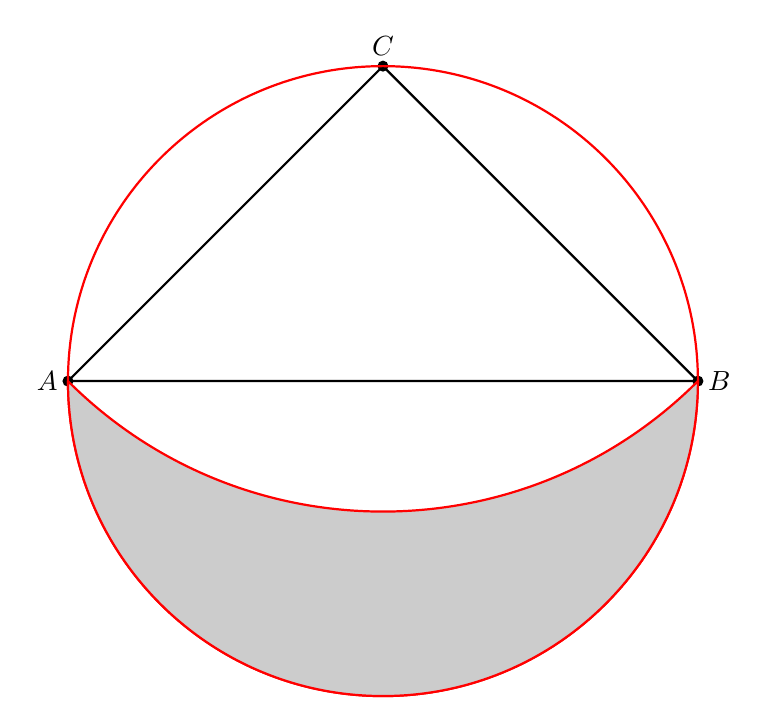
\begin{tikzpicture}[thick]
    \path[draw] (-4,0)  coordinate [label= left:$A$] (A)
            -- ( 0,4)  coordinate [label=above:$C$] (C)
            -- ( 4,0)  coordinate [label=right:$B$] (B)
            -- cycle;
    \foreach \point in {A,B,C}
           \fill [black] (\point) circle (2pt);
    \draw [color=red] circle(4cm);
    % The radius of the inner circular arc is equal to the length of BC.
    % Use the math engine to do the necessary calculations and store the
    % radius in the \n1 register
    \draw[color=red,fill=black!20]
         let \p1 = ($ (B) - (C) $),
             \n1 = {veclen(\x1,\y1)} in
         (A) arc (180:360:4cm) arc (-45:-135:\n1);
\end{tikzpicture}
\end{document}